\begin{greek}
\chapter{Εισαγωγή}\label{ch:intro}

Οι προγραμματιστές στρέφονται ολοένα και περισσότερο σε γλώσσες
και συστήματα εκτέλεσης που παρέχουν αυτόματες υπηρεσίες διαχείρισης,
χάριν των πολλών πλεονεκτημάτων
που αυτά προσφέρουν, όπως η αυξημένη ασφάλεια του κώδικα και
η δυνατότητα προγραμματισμού σε υψηλό αφαιρετικό επίπεδο που δεν
απαιτεί λεπτομερή γνώση του λειτουργικού συστήματος ή/και της
αρχιτεκτονικής. Ο Butters \cite{butt07} διαπιστώνει πώς τα οφέλη
του διαχειριζόμενου κώδικα είναι ευρέως αποδεκτά. Καθώς η εικονική
μηχανή προσφέρει πολλές υπηρεσίες, οι προγραμματιστές χρειάζεται
να γράφουν λιγότερο κώδικα. Ο κώδικας είναι ασφαλέστερος αν περάσει
επιτυχώς έναν (στατικό) έλεγχο τύπων και αν το σύστημα εκτέλεσης
επαληθεύει τον κώδικα καθώς αυτός φορτώνεται, ελέγχει για παραβιάσεις
κατά την πρόσβαση σε πόρους (όπως για παράδειγμα δεικτοδότηση εκτός
ορίων ενός πίνακα) και διαχειρίζεται αυτόματα τη μνήμη. Το κόστος
ανάπτυξης λογισμικού μειώνεται σημαντικά καθώς είναι πλέον ευκολότερη
(αν και όχι πάντα εφικτή) η ανάπτυξη εφαρμογών που δύνανται να
τρέξουν σε διαφορετικές πλατφόρμες. Τα παραπάνω επιτρέπουν στους
προγραμματιστές να αφιερώνουν περισσότερο χρόνο στη λογική των
εφαρμογών.

Σχεδόν όλες οι σύγχρονες γλώσσες προγραμματισμού χρησιμοποιούν
\textbf{δυναμική εκχώρηση μνήμης}. Αυτό επιτρέπει τη δέσμευση
και αποδέσμευση μνήμης για ένα αντικείμενο ακόμη και αν το συνολικό
μέγεθος αυτού δεν ήταν γνωστό κατά τη διάρκεια της μεταγλώττισης
ή η διάρκεια ζωής του ξεπερνά αυτήν της ρουτίνας στην οποία
αυτό εκχωρήθηκε. Ένα αντικείμενο που δημιουργείται δυναμικά
αποθηκεύεται στο \textbf{σωρό} και όχι στη \textbf{στοίβα}
(στο \textbf{εγγράφημα δραστηριοποίησης} της διαδικασίας στην
οποία εκχωρήθηκε) είτε \textbf{στατικά} (δηλαδή σε κάποια διεύθυνση
που είναι γνωστή κατά το χρόνο μεταγλώττισης ή σύνδεσης). Η
εκχώρηση μνήμης στο σωρό είναι ιδιαίτερα σημαντική καθώς επιτρέπει
στον προγραμματιστή:

\begin{itemize}
\item να επιλέξει δυναμικά το μέγεθος νέων αντικειμένων,
\item να ορίσει και να χρησιμοποιήσει αναδρομικές δομές δεδομένων 
      όπως συνδεδεμένες λίστες και δυαδικά δένδρα,
\item να επιστρέφει αντικείμενα στην καλούσα διαδικασία,
\item να επιστρέφει μια συνάρτηση ως αποτέλεσμα μιας συνάρτησης.
\end{itemize}

Η πρόσβαση στα αντικείμενα του σωρού γίνεται μέσω \textbf{αναφορών}.
Τυπικά, μια αναφορά είναι ένας \textbf{δείκτης} προς το αντικείμενο
(και πιο συγκεκριμένα στη διεύθυνση του στη μνήμη). 

\begin{figure}
  \centering
  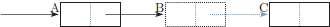
\includegraphics{figures/intro_1}
  \caption[Η πρόωρη διαγραφή ενός αντικειμένου μπορεί να οδηγήσει
           σε σφάλματα]
    {Η πρόωρη διαγραφή ενός αντικειμένου μπορεί να οδηγήσει σε
     σφάλματα. Εδώ η μνήμη του αντικειμένου $B$ έχει ανακτηθεί. Το
     ζωντανό αντικείμενο $A$ περιέχει πλέον έναν ξεκρέμαστο δείκτη.
     Ταυτόχρονα, υπάρχει διαρροή μνήμης: η μνήμη που καταλαμβάνει
     το αντικείμενο $C$ δεν μπορεί να ανακτηθεί παρότι αυτό δεν
     είναι προσβάσιμο.}
   \label{fig:intro_1}  
\end{figure}

\section{Ρητή αποδέσμευση μνήμης}
Κάθε μη τετριμμένο πρόγραμμα το οποίο τρέχει με πεπερασμένη μνήμη
στη διάθεσή του, χρειάζεται κατά καιρούς να επανακτήσει τη μνήμη
που φιλοξενεί αντικείμενα μη χρήσιμα στους υπολογισμούς. Η μνήμη
που χρησιμοποιείται από αντικείμενα του σωρού μπορεί να ανακτηθεί
είτε χρησιμοποιώντας \textbf{ρητή αποδέσμευση} (όπως για παράδειγμα
συμβαίνει με τις συναρτήσεις \textenglish{\textproc{free}} στη γλώσσα C
ή \textenglish{\textproc{delete}} στη γλώσσα C++) είτε αυτόματα από το
\textbf{σύστημα εκτέλεσης}, χρησιμοποιώντας καταμέτρηση αναφορών όπως ο
Collins \cite{DBLP:journals/cacm/Collins60} είτε έναν συλλέκτη σκουπιδιών
εξιχνίασης όπως ο McCarthy \cite{DBLP:journals/cacm/McCarthy60}. Η ρητή
αποδέσμευση μνήμης είναι ευάλωτη σε δύο είδη σφαλμάτων.

Πρώτον, η μνήμη ενός αντικειμένου μπορεί να αποδεσμευθεί πρόωρα και
ενώ υπάρχουν ακόμη αναφορές προς το αντικείμενο. Μία τέτοια αναφορά
ονομάζεται \textbf{ξεκρέμαστος δείκτης}. Το αποτέλεσμα που προκύπτει
αν ένα πρόγραμμα ακολουθήσει έναν τέτοιο δείκτη είναι απρόβλεπτο.
Ο προγραμματιστής δεν έχει κανέναν έλεγχο όσον αφορά το τι συμβαίνει
με την αποδεσμευμένη μνήμη: το σύστημα εκτέλεσης μπορεί να επιλέξει,
μεταξύ άλλων να την καθαρίσει (εγγράψει με μηδενικά), να την
εκχωρήσει για την αποθήκευση ενός νέου αντικειμένου ή να την
επιστρέψει στο λειτουργικό σύστημα. Το καλύτερο σενάριο στο οποίο
μπορεί ο προγραμματιστής να ελπίζει είναι ο βίαιος τερματισμός του
προγράμματος. Είναι ωστόσο πιθανότερο το πρόγραμμα να συνεχίσει
την εκτέλεσή του για εκατομμύρια κύκλους πριν τερματιστεί (καθιστώντας
την αποσφαλμάτωση επίπονη) ή ακόμη και να ολοκληρώσει επιτυχώς
την εκτέλεσή του παράγοντας ωστόσο λανθασμένα αποτελέσματα
(γεγονός που ανιχνεύεται δύσκολα).

Δεύτερον, ο προγραμματιστής μπορεί να αποτύχει να αποδεσμεύσει
τη μνήμη από ένα αντικείμενο το οποίο δε χρειάζεται πια το πρόγραμμα,
οδηγώντας με τον τρόπο αυτό σε \textbf{διαρροή μνήμης}. Σε μικρά
προγράμματα οι διαρροές μπορούν να αγνοηθούν, ωστόσο σε μεγάλα
προγράμματα μπορεί να προκαλέσουν μείωση της επίδοσης (καθώς
ο διαχειριστής μνήμης πασχίζει να ικανοποιήσει αιτήματα εκχώρησης)
είτε σε αποτυχία εκτέλεσης (αν το πρόγραμμα ξεμείνει από μνήμη).
Συχνά μάλιστα μία εσφαλμένη αποδέσμευση μπορεί να προκαλέσει
ταυτόχρονα τόσο ένα ξεκρέμαστο δείκτη όσο και μια διαρροή.

Τα προγραμματιστικά σφάλματα του τύπου αυτού είναι συνήθη σε
περιβάλλοντα όπου δύο ή και περισσότερες διαδικασίες διατηρούν
αναφορές προς το ίδιο αντικείμενο. Η κατάσταση είναι ακόμη πιο
προβληματική σε περιβάλλοντα ταυτόχρονου προγραμματισμού όπου
δύο ή περισσότερα νήματα χειρίζονται δείκτες προς το ίδιο αντικείμενο.

Τι κάνουν λοιπόν οι προγραμματιστές σε μία γλώσσα που δεν υποστηρίζει
αυτόματη δυναμική διαχείριση μνήμης; Η ερώτηση αυτή έχει απασχολήσει
αρκετούς ερευνητές με την επικρατέστερη άποψη να ισχυρίζεται πώς
ο προγραμματιστής απαιτείται να είναι συνεπής όσον αφορά τον τρόπο
με τον οποίο χειρίζεται την \textbf{ιδιοκτησία} των αντικειμένων.
Ο Belotsky \cite{belo03} και άλλοι ερευνητές προτείνουν διαφορετικές
στρατηγικές για τη γλώσσα C++. Αρχικά, οι προγραμματιστές πρέπει
να αποφεύγουν τη δέσμευση μνήμης στο σωρό, όποτε αυτό είναι
δυνατό. Τα αντικείμενα μπορούν να δεσμεύονται στη στοίβα. Και
κατά δεύτερον οι προγραμματιστές θα πρέπει να περνούν σε και να
επιστρέφουν από συναρτήσεις/διαδικασίες αντικείμενα κατά τιμή,
αντιγράφοντας όλα τα περιεχόμενα της παραμέτρου ή του αποτελέσματος
αντί να περνούν δείκτες σε αυτά. Είναι προφανές πώς και οι δύο
προσεγγίσεις αποτρέπουν τα σφάλματα που αφορούν την εκχώρηση και
αποδέσμευση μνήμης αλλά συνοδεύονται από αυξημένη κίνηση μνήμης
και απώλεια δυνατότητας διαμοιρασμού δεδομένων. Σε μερικές περιπτώσεις
επίσης μπορούν να χρησιμοποιηθούν ειδικοί εκχωρητές, οι οποίοι
για παράδειγμα μπορούν να διαχειρίζονται μια δεξαμενή αντικειμένων.
Στο τέλος της φάσης ενός προγράμματος, ολόκληρη η δεξαμενή μπορεί
να αποδεσμεύεται. Στη γλώσσα προγραμματισμού C++ έχουν προταθεί
και υλοποιηθεί ειδικές κλάσεις αντικειμένων δεικτών με σκοπό
την καλύτερη διαχείριση μνήμης.

Η πληθώρα των διαφορετικών στρατηγικών για ασφαλή ρητή διαχείριση
μνήμης δημιουργεί ακόμη ένα πρόβλημα. Ποια προσέγγιση πρέπει
να ακολουθήσει ο προγραμματιστής αν πρέπει να διαχειριστεί με
συνέπεια την ιδιοκτησία των αντικειμένων; Αυτό είναι ιδιαίτερα
δύσκολο να απαντηθεί όταν χρησιμοποιείται κώδικας βιβλιοθήκης.
Προκύπτουν ερωτήματα σχετικά με το ποια προσέγγιση υιοθετεί ο
κώδικας της βιβλιοθήκης και αν όλες οι βιβλιοθήκες που χρησιμοποιεί
το πρόγραμμα υιοθετούν την ίδια προσέγγιση.

\section{Αυτόματη δυναμική διαχείριση μνήμης}
Η αυτόματη διαχείριση μνήμης επιλύει πολλά από τα παραπάνω προβλήματα.
Η \textbf{συλλογή σκουπιδιών} αποτρέπει την εμφάνιση ξεκρέμαστων
δεικτών: ένα αντικείμενο ελευθερώνεται μόνο όταν δεν υπάρχει
κάποιος δείκτης σε αυτό από προσβάσιμο αντικείμενο. Αντίστροφα,
όλα τα μη προσβάσιμα αντικείμενα θα ελευθερωθούν τελικώς από το
συλλέκτη. Όλες οι αποφάσεις σχετικά με την ανάκτηση μνήμης
ανατίθενται στο συλλέκτη, ο οποίος διαθέτει καθολική γνώση της
δομής των αντικειμένων στο σωρό και των νημάτων που έχουν πρόσβαση
σε αυτά.

Η διαχείριση μνήμης είναι ένα θέμα μηχανικής λογισμικού. Τα καλώς
σχεδιασμένα προγράμματα χτίζονται από ψηφίδες (modules) υψηλής
συνεκτικότητας και χαμηλής σύζευξης. Η αύξηση της συνεκτικότητας
και η μείωση της σύζευξης καθιστά ευκολότερη τη συντήρηση των
προγραμμάτων. Ιδανικά, ένας προγραμματιστής θα πρέπει να είναι
σε θέση να καταλαβαίνει τη συμπεριφορά μιας ψηφίδας μόνο από
τον κώδικα της ψηφίδας ή στη χειρότερη περίπτωση και από τον
κώδικα ενός μικρού αριθμού συγγενικών ψηφίδων. Η μείωση της
σύζευξης μεταξύ ψηφίδων πρακτικά σημαίνει πώς η συμπεριφορά
μιας ψηφίδας δεν εξαρτάται από την υλοποίηση κάποιας άλλης ψηφίδας.
Στα πλαίσια της σωστής διαχείρισης μνήμης, αυτό σημαίνει πώς
οι ψηφίδες δεν έχουν γνώση της εσωτερικής λειτουργίας των ψηφίδων
που υλοποιούν τη διαχείριση μνήμης. Η χειρωνακτική διαχείριση
μνήμης αντίθετα δε συμμορφώνεται με τις αρχές της μηχανικής
λογισμικού για ελαχιστοποίηση της επικοινωνίας μεταξύ ψηφίδων.
Το κύριο επιχείρημα υπέρ της αυτόματης διαχείρισης μνήμης δεν
είναι ότι απλοποιεί τη συγγραφή κώδικα (το οποίο ισχύει) αλλά
ότι διαζευγνύει το πρόβλημα της διαχείρισης μνήμης από διαπροσωπείες
αντί να το διασπείρει στον κώδικα. Επίσης διευκολύνει την επαναχρησιμοποίηση
κώδικα. Γι αυτούς τους λόγους η συλλογή σκουπιδιών αποτελεί, άμεσα
ή έμμεσα απαίτηση στο πρότυπο των περισσότερων σύγχρονων γλωσσών
προγραμματισμού. 

Τονίζουμε ωστόσο πώς η συλλογή σκουπιδιών δεν μπορεί να εξαλείψει
πλήρως την εμφάνιση σφαλμάτων που αφορούν τη μνήμη. Οι διαρροές
μνήμης αποτελούν ένα από πιο συχνά εμφανιζόμενα σφάλματα μνήμης.
Παρότι η συλλογή σκουπιδιών τείνει να μειώσει την εμφάνιση διαρροών
μνήμης, δεν μπορεί να εγγυηθεί την πλήρη εξάλειψή τους. Εάν ένα
αντικείμενο δεν είναι πλέον προσβάσιμο από το υπόλοιπο πρόγραμμα,
ο συλλέκτης θα ανακτήσει τη μνήμη που αυτό καταλαμβάνει. Εφόσον
αυτός είναι ο μόνος τρόπος με τον οποίο ένα αντικείμενο μπορεί
να διαγραφεί, δεν μπορούν να προκύψουν ξεκρέμαστοι δείκτες.
Επιπλέον, αν η διαγραφή ενός αντικειμένου καθιστά και τα αντικείμενα
παιδιά του μη προσβάσιμα, τότε ο συλλέκτης θα ανακτήσει και τη
μνήμη που αυτά καταλαμβάνουν. Ωστόσο, ο συλλέκτης δεν μπορεί να
βοηθήσει κάπως αν υπάρχει μια δυναμική δομή δεδομένων η οποία
συνεχώς αυξάνεται (για παράδειγμα επειδή ο προγραμματιστής εσφαλμένα
μόνο προσθέτει σε αυτή δεδομένα χωρίς ποτέ να αφαιρεί) ή αν αυτή
είναι μεν προσβάσιμη από το υπόλοιπο πρόγραμμα αλλά αυτό δε θα
τη χρησιμοποιήσει ποτέ στο μέλλον.

\begin{table}
  \centering
  \begin{tabular}{|l|l|l|}
    \hline
    ActionScript (2000) & Algol-68 (1965)   & APL (1964)\\
    AppleScript (1993)  & AspectJ (2001)    & Awk (1977)\\
    Beta (1983)         & C\# (1999)        & Cyclone (2006)\\
    Managed C++ (2002)  & Cecil (1992)      & Cedar (1983)\\
    Clean (1984)        & CLU (1974)        & D (2007)\\
    Dylan (1992)        & Dynace (1993)     & E (1997)\\
    Eiffel (1986)       & Elasti-C (1997)   & Emerald (1988)\\
    Erlang (1990)       & Euphoria (1993)   & F\# (2005)\\ 
    Fortress (2006)     & Green (1998)      & Go (2010)\\
    Groovy (2004)       & Haskell (1990)    & Hope (1978)\\
    Icon (1977)         & Java (1994)       & JavaScript (1994)\\
    Liana (1991)        & Limbo (1996)      & Lingo (1991)\\
    LotusScript (1995)  & Lua (1994)        & Mathematica (1987)\\
    MATLAB (1970s)      & Mercury (1993)    & Miranda (1985)\\
    ML (1990)           & Modula-3 (1988)   & Oberon (1985)\\
    Objective-C (2007-) & Obliq (1993)      & Perl (1986)\\
    Pike (1996)         & PHP (1995)        & Pliant (1999)\\
    POP-2 (1970)        & PostScript (1982) & Prolog (1982)\\
    Python (1991)       & Rexx (1979)       & Ruby (1993)\\
    Sather (1990)       & Scala (2003)      & Scheme (1975)\\
    Self (1986)         & SETL (1969)       & Simula (1964)\\
    SISAL (1983)        & Smalltalk (1972)  & SNOBOL (1962)\\
    Squeak (1996)       & Tcl (1990)        & Theta (1994)\\
    VB.NET (2001)       & VBScript (1996)   & Visual Basic (1991)\\
    VHDL (1987)         & X10 (2004)        & YAFL (1993)\\
    \hline
  \end{tabular}
  \caption
    [Γλώσσες προγραμματισμού και συλλογή σκουπιδιών]
    {Γλώσσες προγραμματισμού και συλλογή σκουπιδιών. Όλες οι
     παραπάνω γλώσσες βασίζονται σε συλλογή σκουπιδιών.}
  \label{tab:intro_1}
\end{table}

\section{Συγκρίνοντας αλγορίθμους συλλογής σκουπιδιών}
Η παρούσα εργασία εξετάζει μια ευρεία γκάμα αλγορίθμων για συλλογή
σκουπιδιών, κάθε ένας από τους οποίους έχει σχεδιασθεί λαμβάνοντας
υπόψιν διαφορετικές απαιτήσεις όσον αφορά το φορτίο εργασίας,
το υλικό και τις επιδόσεις. Δυστυχώς, δεν υπάρχει κάποιος αλγόριθμος
που λειτουργεί βέλτιστα σε όλες τις περιπτώσεις. Οι Fitzgerald
και Tarditi \cite{DBLP:conf/iwmm/FitzgeraldT00} μελετώντας 6 
διαφορετικούς συλλέκτες και 20 benchmarks διαπίστωσαν πώς για
κάθε συλλέκτη υπάρχει τουλάχιστον ένα benchmark το οποίο θα εκτελούνταν
τουλάχιστον 15\% ταχύτερα με την παρουσία ενός πιο κατάλληλου
συλλέκτη. Ο Singer κ.ά. \cite{DBLP:conf/iwmm/SingerBWC07} εφαρμόζουν
τεχνικές μηχανικής μάθησης προκειμένου να προβλέψουν βέλτιστη
διαμόρφωση ενός συλλέκτη για ένα συγκεκριμένο πρόγραμμα. Άλλοι
ερευνητές \cite{DBLP:conf/jvm/Printezis01,DBLP:conf/iwmm/SomanKB04}
έχουν εξερευνήσει την ιδέα να επιτρέπουν στις εικονικές μηχανές
Java να αλλάζουν συλλέκτη καθώς εκτελούνται εάν πιστεύουν, με
βάση τα χαρακτηριστικά του υπό εκτέλεση προγράμματος πώς αυτό
θα ωφεληθεί από την παρουσία ενός διαφορετικού συλλέκτη. Στην
ενότητα αυτή παρουσιάζουμε τις μετρικές βάση των οποίων συγκρίνονται
οι διαφορετικοί αλγόριθμοι συλλογής σκουπιδιών. Τονίζουμε ωστόσο
πώς οι μετρικές αυτές δεν είναι ανεξάρτητες μεταβλητές: η ρύθμιση
μιας παραμέτρου με σκοπό την επίτευξη ενός συγκεκριμένου στόχου
ενδέχεται να προκαλέσει άλλες αντιφατικές επιδράσεις.

\subsection{Ασφάλεια}
Ένας αλγόριθμος συλλογής σκουπιδιών πρέπει καταρχήν να είναι
\textbf{ασφαλής}: δεν πρέπει ποτέ να ανακτήσει τη μνήμη αντικειμένων
που είναι ζωντανά. Η εξασφάλιση της ασφάλειας είναι ιδιαίτερα
δύσκολη σε ταυτόχρονους συλλέκτες. Επίσης η ασφάλεια της
\textbf{συντηρητικής συλλογής σκουπιδιών}, όπου ο συλλέκτης δεν
έχει καμία απολύτως βοήθεια από το μεταγλωττιστή και το σύστημα
εκτέλεσης, είναι ευάλωτη σε συγκεκριμένες βελτιστοποιήσεις του
μεταγλωττιστή οι οποίες έχουν ως αποτέλεσμα δεδομένα που
δεν είναι δείκτες να φαίνεται ότι είναι.

\subsection{Ρυθμαπόδοση}
Κοινή απαίτηση των χρηστών είναι τα προγράμματά τους να τρέχουν
ταχύτερα. Για να συμβαίνει αυτό, πρέπει μεταξύ άλλων, ο υπολογιστικός
χρόνος που αφορά συλλογή σκουπιδιών να είναι ο ελάχιστος δυνατός.
Στις περισσότερες περιπτώσεις βέβαια, ο χρήστης ενδιαφέρεται το
σύνολο της εφαρμογής (τροποποιητής και συλλέκτης) να εκτελείται
σε όσο το δυνατόν λιγότερο χρόνο. Στα περισσότερα καλώς σχεδιασμένα
συστήματα, ξοδεύεται πολύ περισσότερος χρόνος CPU για την εκτέλεση
του τροποποιητή από ότι για την εκτέλεση του συλλέκτη. Έτσι πολλές
φορές αξίζει να θυσιαστεί η επίδοση του συλλέκτη χάριν υψηλότερης 
διεκπεραιωτικής ικανότητας του τροποποιητή.

\subsection{Πληρότητα και προθυμία}
Ιδανικά, η συλλογή σκουπιδιών οφείλει να είναι \textbf{πλήρης}: 
τελικώς όλα τα σκουπίδια στο σωρό θα συλλεγούν. Ωστόσο, αυτό
δεν είναι πάντοτε δυνατό ή και επιθυμητό. Όπως θα δούμε και στο
κεφάλαιο~\ref{ch:refcnt}, οι απλοϊκοί αλγόριθμοι καταμέτρησης
αναφορών για παράδειγμα αδυνατούν να συλλέξουν αυτοαναφορικές
δομές δεδομένων. Επιπλέον, για λόγους επίδοσης, μπορεί να είναι 
επιθυμητό να μη συλλεγεί ολόκληρος ο σωρός σε κάθε κύκλο συλλογής.
Οι γενεαλογικοί συλλέκτες για παράδειγμα, διαχωρίζουν τα αντικείμενα
με βάση την ηλικία τους σε δύο ή περισσότερες περιοχές του σωρού
τις οποίες ονομάζουν γενεές. Επικεντρώνοντας την προσοχή τους στη
νεότερη γενιά, οι γενεαλογικοί συλλέκτες βελτιώνουν τόσο το συνολικό
χρόνο εκτέλεσης του συλλέκτη όσο και το μέσο χρόνο παύσης του
τροποποιητή για την κάθε ξεχωριστή ενεργοποίηση αυτού. 

Οι ταυτόχρονοι συλλέκτες αναμιγνύουν την εκτέλεση τροποποιητή
και συλλέκτη με στόχο την αποφυγή ή έστω τη μείωση της χρονικής
διάρκειας των διακοπών του προγράμματος χρήστη. Μια συνέπεια
αυτού είναι πώς τα αντικείμενα που έχουν γίνει σκουπίδια αφού
έχει ξεκινήσει ένας κύκλος συλλογής μπορεί να μην ελευθερωθούν
παρά στο τέλος του επόμενου κύκλου. Τέτοια αντικείμενα ονομάζονται
\textbf{αιωρούμενα σκουπίδια}. Σε ένα περιβάλλον λοιπόν όπου
συλλέκτης και τροποποιητής εκτελούνται ταυτόχρονα η πληρότητα
του συλλέκτη σχετίζεται με την \textbf{τελική} συλλογή των σκουπιδιών. 
Διαφορετικοί αλγόριθμοι μπορεί να διαφέρουν ως προς την 
\textbf{προθυμία} συλλογής τους, οδηγώντας σε συμβιβασμούς χώρου
/χρόνου. 

\subsection{Χρόνος παύσης}
Μια σημαντική απαίτηση συνήθως είναι η ελαχιστοποίηση της εισβολής
του συλλέκτη στην εκτέλεση του προγράμματος. Πολλοί συλλέκτες
εισάγουν παύσεις στην εκτέλεση ενός προγράμματος καθώς όλα τα
νήματα του τροποποιητή είναι σταματημένα την ώρα που αυτοί συλλέγουν
σκουπίδια. Ο όρος \textbf{παύση του κόσμου} αναφέρεται ακριβώς
στην αναστολή της εκτέλεσης των νημάτων τροποποιητών κατά τη
διάρκεια της εκτέλεσης των νημάτων συλλεκτών. Είναι εμφανώς
επιθυμητό οι \textbf{χρόνοι παύσης} να ελαχιστοποιηθούν. Αυτό
μπορεί να είναι ιδιαίτερα σημαντικό για διαδραστικές εφαρμογές
ή διακομιστές οι οποίοι χειρίζονται συναλλαγές (όπου συνήθως οι
ενέργειες πρέπει να διεκπεραιώνονται εντός πολύ στενών χρονικών
ορίων). Ωστόσο, οι μηχανισμοί που προσπαθούν να μειώσουν τους
χρόνους παύσης έχουν παρενέργειες όπως θα δούμε στη συνέχεια.
Για παράδειγμα οι γενεαλογικοί συλλέκτες προσπαθούν να μειώσουν
τους χρόνους παύσης συλλέγοντας συχνά και γρήγορα μία μικρή
περιοχή του σωρού που φιλοξενεί νέα αντικείμενα ενώ συλλέγουν
μεγαλύτερες περιοχές του σωρού όπου ζουν παλαιά αντικείμενα
σπανιότερα και μόνο αν αυτό χρειασθεί. Ωστόσο, επειδή πρέπει
να καταγράφονται οι δείκτες που περνούν τα όρια των περιοχών,
η γενεαλογική συλλογή σκουπιδιών επιβάλλει ένα μικρό πρόστιμο
στις λειτουργίες εγγραφής δεικτών του τροποποιητή.

Οι παράλληλοι συλλέκτες σταματούν τα νήματα του τροποποιητή και
μειώνουν το χρόνο παύσης απασχολώντας πολλά νήματα. Οι αυξητικοί
και ταυτόχρονοι συλλέκτες επιχειρούν να μειώσουν τους χρόνους
παύσης ακόμη περισσότερο εκτελώντας ένα μικρό κβάντο εργασιών
συλλογής είτε ανάμεσα στις λειτουργίες του τροποποιητή είτε
παράλληλα με αυτές. Και αυτές οι τεχνικές υπαγορεύουν ένα μικρό
κόστος στον τροποποιητή προκειμένου να επιτευχθεί ο σωστός συγχρονισμός 
αυτού με το συλλέκτη.

Η μέγιστη τιμή ή ο μέσος χρόνος παύσης ωστόσο δεν μπορούν να
χρησιμοποιηθούν ώστε να ελεγχθεί η πρόοδος του τροποποιητή. Η
κατανομή των χρόνων παύσης είναι επίσης μια μετρική που ενδιαφέρει.
Στη βιβλιογραφία συναντώνται διάφοροι τρόποι μέτρησης αυτής,
όπως η \textbf{ελάχιστη χρησιμοποίηση τροποποιητή} \cite{DBLP:conf/pldi/ChengB01},
και η \textbf{φραγμένη χρησιμοποίηση τροποποιητή} \cite{DBLP:conf/oopsla/SachindranMB04}.
Και οι δύο μετρικές προσπαθούν να μετρήσουν με ακρίβεια το
ελάχιστο κλάσμα του χρόνου εκτέλεσης που δαπανάται για την
εκτέλεση του τροποποιητή.

\subsection{Επιβάρυνση σε χώρο}
Ο στόχος ενός διαχειριστή μνήμης είναι η ασφαλής και αποδοτική
χρήση του χώρου. Διαφορετικοί διαχειριστές, τόσο ρητοί όσο και
αυτόματοι επιβάλλουν διαφορετικά \textbf{χωρικά κόστη}. Οι συλλέκτες
με καταμέτρηση αναφορών για παράδειγμα χρειάζονται χώρο στη
μνήμη κάθε αντικειμένου όπου θα αποθηκεύεται ο μετρητής αναφορών
προς αυτό. Οι συλλέκτες με σήμανση και εκκαθάριση αποθηκεύουν
ένα bit/byte στην επικεφαλίδα ενός αντικειμένου, ενώ κάποιοι
συλλέκτες με σήμανση και συμπύκνωση αποθηκεύουν τη νέα διεύθυνση
ενός αντικειμένου σε κάποιο πεδίο στο παλαιό αντίγραφο αυτού.
Οι συλλέκτες αντιγραφής διαχωρίζουν το σωρό σε δύο ημιχώρους,
μόνο ένας εκ των οποίων είναι διαθέσιμος στον τροποποιητή κάθε
χρονική στιγμή: ο άλλος χρησιμεύει ως αντίγραφο ρεζέρβα όπου
ο συλλέκτης θα αντιγράψει τα ζωντανά αντικείμενα στη διάρκεια
του επόμενου κύκλου συλλογής. Οι συλλέκτες ενδέχεται επίσης να
χρησιμοποιούν βοηθητικές δομές δεδομένων. Οι ταυτόχρονοι συλλέκτες,
ή οι γενεαλογικοί συλλέκτες απαιτούν τη χρήση ενθυμούμενων συνόλων
ώστε να καταγράφουν τις τιμές ποιων δεικτών έχει μεταβάλλει στο
ενδιάμεσο ο τροποποιητής ή τις διευθύνσεις των διαγενεαλογικών
δεικτών αντίστοιχα.

\subsection{Βελτιστοποιήσεις για ειδικές γλώσσες}
Οι αλγόριθμοι συλλογής σκουπιδιών πολλές φορές χαρακτηρίζονται
από την εφαρμοσιμότητά τους σε γλώσσες προγραμματισμού διαφορετικών
οικογενειών. Οι συναρτησιακές γλώσσες για παράδειγμα προσφέρονται
για βελτιστοποιήσεις που σχετίζονται με την αυτόματη διαχείριση
μνήμης. Μερικές γλώσσες, όπως η ML διακρίνουν τα δεδομένα σε
τροποποιήσιμα και μη τροποποιήσιμα. Αγνές συναρτησιακές γλώσσες
όπως η Haskell, επεκτείνουν την παραπάνω ιδέα και δεν αφήνουν
τον προγραμματιστή να τροποποιήσει καμία τιμή (τα προγράμματα
χαρακτηρίζονται από διαφάνεια αναφορών). Εσωτερικά ωστόσο, ενημερώνουν
δομές δεδομένων τουλάχιστον μια φορά, κάτι που δίνει τη δυνατότητα
σε γενεαλογικούς συλλέκτες σκουπιδιών να προάγουν πρόθυμα πλήρως
υπολογισμένες δομές δεδομένων. Έχουν επίσης προταθεί \textbf{πλήρεις}
μηχανισμοί για τη συλλογή κύκλων σκουπιδιών με καταμέτρηση αναφορών.
Οι δηλωτικές γλώσσες προγραμματισμού ενδεχομένως επιτρέπουν τη
χρήση μηχανισμών για αποδοτική διαχείριση του σωρού. Όλα τα δεδομένα
που έχουν δημιουργηθεί μετά από ένα σημείο επιλογής σε μία γλώσσα
λογικού προγραμματισμού καθίστανται μη προσβάσιμα τη χρονική
στιγμή κατά την οποία το πρόγραμμα οπισθοχωρεί στο εν λόγω σημείο.
Εάν ο διαχειριστής μνήμης διατάσσει τα αντικείμενα στο σωρό με
βάση τη σειρά δημιουργίας τους, η συνολική μνήμη που έχει εκχωρηθεί
από το σημείο επιλογής και έπειτα μπορεί να επιστραφεί σε σταθερό
χρόνο. Αντίστροφα, διαφορετικά πρότυπα γλωσσών μπορεί να ορίζουν
συγκεκριμένες απαιτήσεις από το συλλέκτη. Οι πιο γνωστές αφορούν
την ικανότητα του συλλέκτη να χειρίζεται διάφορα είδη δεικτών
ή να προκαλεί την οριστικοποίηση (finalization) νεκρών αντικειμένων. 

\subsection{Κλιμακωσιμότητα και μεταφερσιμότητα}
Η ολοένα και περισσότερο αυξανόμενη διάδοση πολυπύρηνων επεξεργαστών
σε επιτραπέζιους και φορητούς υπολογιστές πέραν των διακομιστών
μεγάλης κλίμακας καθιστά ιδιαίτερα σημαντική την ανάγκη η συλλογή
σκουπιδιών να επωφεληθεί από την παρουσία του παράλληλου υλικού.
Έτσι συχνά ένας αλγόριθμος συλλογής σκουπιδιών χαρακτηρίζεται
ως προς το πώς \textbf{κλιμακώνει}. Η λειτουργία ενός αριθμού
αλγορίθμων συλλογής σκουπιδιών εξαρτάται από την υποστήριξη που
παρέχει το λειτουργικό σύστημα και η αρχιτεκτονική. Αυτό έχει
ως αποτέλεσμα η \textbf{μεταφερσιμότητα} των αλγορίθμων να μην
είναι απαραίτητα εγγυημένη.

\section{Ορολογία}
Στην ενότητα αυτή εξηγούμε την ορολογία που χρησιμοποιείται
στην εργασία αυτή αλλά και στη βιβλιογραφία.

Ο \textbf{σωρός} είναι είτε ένας συνεχόμενος πίνακας από λέξεις
μνήμης ή ένα σύνολο από μη συνεχόμενα μπλοκ συνεχόμενων λέξεων.
Ένα \textbf{αντικείμενο} είναι ένα σύνολο από συνεχόμενες λέξεις
μνήμης. Οι επιμέρους λέξεις ενός αντικείμενου αναφέρονται και ως
\textbf{πεδία}. Σε κάθε πεδίο ενός αντικειμένου αποθηκεύεται ένα
βαθμωτό μέγεθος (π.χ.\ ένας ακέραιος) ή μια \textbf{αναφορά}. Μια
αναφορά είναι είτε ένας δείκτης προς ένα αντικείμενο του σωρού
είτε η ειδική τιμή \textbf{null}. Ένα αντικείμενο συνήθως έχει
ένα ειδικό πεδίο, την \textbf{επικεφαλίδα}, όπου αποθηκεύονται
μεταδεδομένα χρήσιμα για το σύστημα εκτέλεσης. Ο σωρός συχνά
αναφέρεται και ως \textbf{γράφος αντικειμένων}. Ο γράφος είναι
κατευθυνόμενος, με κόμβους τα αντικείμενα του σωρού και ακμές
τους δείκτες στα πεδία αυτών. Μια ακμή αναπαριστά μια αναφορά από
έναν κόμβο αφετηρίας ή μία \textbf{ρίζα} προς έναν κόμβο προορισμού.

\begin{figure}
 \centering
 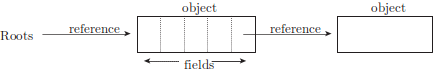
\includegraphics{figures/intro_3}
 \caption[Ρίζες, αναφορές, αντικείμενα, πεδία]
   {Ρίζες, αναφορές, αντικείμενα, πεδία.}
 \label{fig:intro_3}
\end{figure}
 
Σύμφωνα με τον Dijkstra \cite{DBLP:conf/ac/DijkstraLMSS75,
DBLP:journals/cacm/DijkstraLMSS78}, ένα πρόγραμμα με συλλογή
σκουπιδιών διαχωρίζεται στα εξής δύο ημιανεξάρτητα τμήματα:

\begin{itemize}
\item Ο \textbf{τροποποιητής} εκτελεί τον κώδικα της εφαρμογής,
      ο οποίος δημιουργεί αντικείμενα και τροποποιεί το γράφο
      αντικειμένων μεταβάλλοντας αναφορές ώστε αυτές να αναφέρονται
      σε διαφορετικά αντικείμενα προορισμού. Μια αναφορά μπορεί
      να περιέχεται στο πεδίο ενός αντικειμένου ή στις ρίζες
      του προγράμματος (στατικές μεταβλητές, καταχωρητές, στοίβα).
      Καθώς ο τροποποιητής τροποποιεί τις αναφορές, κάθε αντικείμενο
      μπορεί να αποσυνδεθεί από τις ρίζες, δηλαδή να μην είναι
      πλέον προσβάσιμο ακολουθώντας μια ακολουθία αναφορών από
      αυτές.
\item Ο \textbf{συλλέκτης} εκτελεί κώδικα συλλογής σκουπιδιών,
      ο οποίος ανακαλύπτει μη προσβάσιμα αντικείμενα και ανακτά
      τη μνήμη που αυτά καταλαμβάνουν.
\end{itemize}

Ο τροποποιητής μπορεί να είναι είτε \textbf{μονονηματικός}
είτε \textbf{πολυνηματικός}. Το ίδιο ισχύει και για το συλλέκτη.

Εκτός από το σωρό, θεωρούμε πώς υπάρχει ένα (πεπερασμένο) σύνολο
ριζών, το οποίο αναπαριστά δείκτες που είναι \textbf{άμεσα}
προσβάσιμοι από τον τροποποιητή. Κατά επέκταση, τα αντικείμενα
του σωρού στα οποία αναφέρονται οι ρίζες ονομάζονται
\textbf{αντικείμενα ρίζες}. Καθώς ο τροποποιητής εκτελείται,
οι ρίζες και άρα και ο γράφος αντικειμένων μεταβάλλονται.

Αναφερόμαστε σε έναν κόμβο του σωρού $N$ χρησιμοποιώντας τη
διεύθυνσή του στη μνήμη (η οποία δεν αντιστοιχεί απαραίτητα
στην πρώτη λέξη του αντικειμένου αλλά ίσως σε κάποιο προκαθορισμένο
σημείο ανάμεσα στα δεδομένα και τα μεταδεδομένα του αντικειμένου).
Δοθέντος ενός αντικειμένου $N$, αναφερόμαστε στο $i$-στό πεδίο
του, στο οποίο μπορεί να αποθηκεύεται μία βαθμωτή μεταβλητή ή
ένας δείκτης, ως $N[i]$, αντιμετωπίζοντας το αντικείμενο ως
έναν πίνακα από πεδία. Συμβολίζουμε με $|N|$ το πλήθος των
πεδίων ενός αντικειμένου, ενώ η αποδιευθυνσιοδότηση ενός
μη μηδενικού δείκτη $p$ συμβολίζεται με $*p$. Επιπλέον η διεύθυνση
του $i$-στού πεδίου του αντικειμένου $N$ συμβολίζεται με
$\&N[i]$. Επομένως το σύνολο των διευθύνσεων των πεδίων δεικτών
ενός αντικειμένου $N$, συμβολιζόμενο ως $Pointers(N)$ ορίζεται
αυστηρά ως:

$Pointers(N)=\{a | a=\&N[i], \forall i: 0 \leq i < |N| \; where \; N[i] \; is \; a \; pointer\}$

Τέλος, θεωρούμε το σύνολο $Roots$ των ριζών θεωρούμε ως ένα
ψευδοαντικείμενο και αναφερόμαστε στην $i$-στή ρίζα ως $Roots[i]$.

Λέμε πώς ένα αντικείμενο είναι \textbf{ζωντανό} εάν αυτό πρόκειται
να χρησιμοποιηθεί κάποια χρονική στιγμή στο μέλλον από τον τροποποιητή.
Ένας συλλέκτης σκουπιδιών είναι ορθός αν και μόνο αν ποτέ δε
συλλέγει ζωντανά αντικείμενα. Δυστυχώς ωστόσο, η ζωντάνια είναι
μια μη-αποκρίσιμη ιδιότητα των προγραμμάτων: δεν υπάρχει κάποιος
τρόπος ώστε να απαντηθεί αν ένα τυχαίο πρόγραμμα θα χρησιμοποιήσει
ή όχι στο μέλλον ένα αντικείμενο στο σωρό. Το γεγονός πώς ένα
πρόγραμμα διαθέτει ένα δείκτη προς ένα αντικείμενο δε σημαίνει
απαραίτητα και πώς αυτό θα προσπελαστεί από το πρόγραμμα κάποια
στιγμή στο μέλλον. Προσεγγίζουμε τη ζωντάνια με την αποκρίσιμη
ιδιότητα της \textbf{προσβασιμότητα μέσω δεικτών}. Ένα αντικείμενο
$N$ είναι προσβάσιμο από ένα αντικείμενο $M$, εάν το $N$ μπορεί
να προσπελασθεί ακολουθώντας μία ακολουθία δεικτών από κάποιο
πεδίο $f$ του $M$. Επομένως, ένα αντικείμενο είναι προσβάσιμο
από τις ρίζες ενός τροποποιητή αν και μόνο αν υπάρχει μια ακολουθία
δεικτών που ξεκινάει από κάποια ρίζα και καταλήγει σε αυτό.

Πιο αυστηρά, ορίζουμε την δυαδική σχέση $\rightarrow_f$ ως εξής.
Για κάθε δύο κόμβους $M, N$, ισχύει πώς $M\rightarrow_f N$ αν
και μόνο εάν υπάρχει ένα πεδίο $f = \& M[i]$, τέτοιο ώστε
$f \in Pointers(M)$ και $*f = N$. Παρόμοια, $Roots \rightarrow_f N$
αν και μόνο αν υπάρχει ένα πεδίο $f$ τέτοιο ώστε $f \in Roots$
και $*f = N$. Λέμε πώς ο κόμβος $N$ είναι \textbf{άμεσα προσβάσιμος}
από τον κόμβο $M$, και συμβολίζουμε με $M \rightarrow N$ αν υπάρχει
κάποιο πεδίο $f$ το οποίο ανήκει στο σύνολο $Pointers(M)$ και είναι
τέτοιο ώστε $M \rightarrow_f N$. Με τη βοήθεια των παραπάνω ορισμών,
το σύνολο των προσβάσιμων αντικειμένων στο σωρό ορίζεται ως το
μεταβατικό κλείσιμο από το σύνολο $Roots$ ως προς την πράξη
$\rightarrow$, δηλαδή το ελάχιστο σύνολο:

$reachable = \{ N \in Nodes \mid (\exists r \in Roots: r \rightarrow N) \lor (\exists M \in reachable: M \rightarrow N) \}$

Ένα αντικείμενο του σωρού που είναι μη προσβάσιμο από τις ρίζες
δε θα προσπελασθεί ποτέ ξανά από έναν ορθό τροποποιητή. Αντίθετα,
ένα προσβάσιμο αντικείμενο μπορεί να προσπελασθεί κάποια στιγμή
στο μέλλον. Με τον τρόπο αυτό η ζωντάνια των αντικειμένων όσον
αφορά τη συλλογή σκουπιδιών, ορίζεται μέσω της προσβασιμότητας
μέσω δεικτών. Τα μη προσβάσιμα αντικείμενα είναι σίγουρα νεκρά
και επομένως μπορούν με ασφάλεια να ελευθερωθούν. Αντίθετα,
τα προσβάσιμα αντικείμενα μπορεί να είναι ζωντανά και επομένως
πρέπει να διατηρηθούν. Παρότι δεν είναι ακριβώς ορθό, θα χρησιμοποιούμε
τους όρους \textbf{ζωντανό} και \textbf{νεκρό} αδιακρίτως με
τους όρους \textbf{προσβάσιμο} και \textbf{μη-προσβάσιμο} αντίστοιχα. 
Τέλος, ο όρος \textbf{σκουπίδι} θα χρησιμοποιείται ως συνώνυμος
του όρου μη-προσβάσιμο.

Ο \textbf{εκχωρητής}, ο οποίος μπορεί να θεωρηθεί λειτουργικά
κάθετος ως προς το συλλέκτη, υποστηρίζει δύο λειτουργίες:
\textenglish{\textproc{allocate}}, η οποία δεσμεύει τη μνήμη που θα καταλάβει
ένα αντικείμενο και \textenglish{\textproc{deallocate}}, η  οποία επιστρέφει
τη μνήμη στον εκχωρητή ώστε αυτός να την επαναχρησιμοποιήσει.

Ορισμένες από τις λειτουργίες που εκτελούν τα νήματα του τροποποιητή
ενδιαφέρουν το συλλέκτη: \textenglish{\textproc{New}}, \textenglish{\textproc{Read}} και
\textenglish{\textproc{Write}}. Συγκεκριμένοι διαχειριστές μνήμης μπορεί να
επεκτείνουν αυτές τις βασικές λειτουργίες και να τις μετατρέπουν
σε \textbf{φράγματα}: πράξεις που επιτρέπουν τη σύγχρονη
ή ασύγχρονη επικοινωνία με το συλλέκτη. Διακρίνουμε τα φράγματα
σε \textbf{φράγματα εγγραφής} και \textbf{φράγματα ανάγνωσης}.

\begin{algorithm}
  \caption{Λειτουργίες τροποποιητή}
  \label{alg:intro1}
  \begin{algorithmic}[1]
    \Function{New}{\null}
      \State \Return{\Call{allocate}{\null}}
    \EndFunction
    \Statex
    \Function{Read}{$src$, $i$}
      \State \Return $src[i]$
    \EndFunction
    \Statex
    \Procedure{Write}{$src$, $i$, $ref$}
      \State $src[i] \gets ref$
    \EndProcedure
  \end{algorithmic}
\end{algorithm}

Στα πλαίσια της ταυτόχρονης εκτέλεσης νημάτων τροποποιητών
και νημάτων συλλεκτών, όλοι οι αλγόριθμοι συλλογής σκουπιδιών
που εξετάζουμε απαιτούν ορισμένες ακολουθίες εντολών να
εκτελούνται \textbf{ατομικά}. Για λόγους απλοποίησης αγνοούμε
τον εκάστοτε μηχανισμό που εξασφαλίζει την ατομική εκτέλεση
τμημάτων κώδικα και απλώς σημειώνουμε τα τελευταία με τη λέξη
κλειδί \textbf{atomic}. 

\section{Οργάνωση της εργασίας}
Στο κεφάλαιο αυτό εξηγούνται οι λόγοι για τους οποίους είναι
επιθυμητή η αυτόματη διαχείριση μνήμης και ορίζονται οι
έννοιες του εκχωρητή μνήμης, του συλλέκτη σκουπιδιών και του
τροποποιητή. Επίσης παρουσιάζονται τα κριτήρια με τα οποία
μπορούν να συγκριθούν οι διαφορετικές στρατηγικές συλλογής
σκουπιδιών. Το υπόλοιπο της εργασίας οργανώνεται σε δύο μέρη.

Το πρώτο μέρος περιλαμβάνει 4 κεφάλαια στα οποία εξετάζονται
με λεπτομέρεια οι θεμελιώδεις αλγόριθμοι συλλογής σκουπιδιών.
Πιο συγκεκριμένα, το κεφάλαιο~\ref{ch:mrkswp} πραγματεύεται τη
συλλογή σκουπιδιών με σήμανση και εκκαθάριση, το κεφάλαιο~\ref{ch:mrkcmp}
τη συλλογή σκουπιδιών με σήμανση και συμπύκνωση, το κεφάλαιο~\ref{ch:cop}
τη συλλογή σκουπιδιών με αντιγραφή και τέλος το κεφάλαιο~\ref{ch:refcnt}
τη συλλογή σκουπιδιών με καταμέτρηση αναφορών.  

Το δεύτερο μέρος της εξετάζει προηγμένους αλγορίθμους συλλογής
σκουπιδιών. και αποτελείται επίσης από 4 κεφάλαια. Το κεφάλαιο~\ref{ch:gen}
πραγματεύεται λεπτομερώς τη γενεαλογική συλλογή σκουπιδιών, το
κεφάλαιο~\ref{ch:par} την παράλληλη συλλογή σκουπιδιών και το
κεφάλαιο~\ref{ch:conc} την ταυτόχρονη συλλογή σκουπιδιών. Τέλος,
στο κεφάλαιο~\ref{ch:rt} δίνεται μια σύντομη εισαγωγή στη
συλλογή σκουπιδιών πραγματικού χρόνου.

\end{greek}
